
%(BEGIN_QUESTION)
% Copyright 2009, Tony R. Kuphaldt, released under the Creative Commons Attribution License (v 1.0)
% This means you may do almost anything with this work of mine, so long as you give me proper credit

Qualitatively graph the response of an {\it integral-only} controller over time to the changes in process variable and setpoint shown here:

$$\includegraphics[width=15.5cm]{i03763x01.eps}$$

Assume {\it direct} control action.

\vskip 20pt \vbox{\hrule \hbox{\strut \vrule{} {\bf Suggestions for Socratic discussion} \vrule} \hrule}

\begin{itemize}
\item{} A handy rule for plotting the output of a proportional-only controller is that the output will always return to the bias value when PV=SP.  Is this rule true for integral controllers as well?  Why or why not?
\item{} Explain how the output trend would look different if the time period of the second error (where SP steps away from PV) were longer in duration.
\end{itemize}

\underbar{file i03763}
%(END_QUESTION)





%(BEGIN_ANSWER)

The controller output graph shown here is {\it qualitative} only.  Although drawn to scale (i.e. all changes in the output are properly scaled relative to each other), the scale itself is arbitrary and therefore may not match the scale of your sketch:

$$\includegraphics[width=15.5cm]{i03763x02.eps}$$

%(END_ANSWER)





%(BEGIN_NOTES)


%INDEX% Control, integral: graphing controller response

%(END_NOTES)


